\glsresetall
\chapter{Metodologia de Avaliação}
Neste capítulo, será apresentado como a solução foi avaliada. Particularmente, as perguntas que guiaram o desenvolvimento dos experimentos desenvolvidos para analisar a virtualização e a migração de processos no \nanvix foram:

\begin{enumerate}[label=(\roman*)]
    \item Qual o impacto do isolamento da \uarea e do código e dados de usuário sobre a execução do \nanvix?
    \item Qual a eficiência da migração de processos no \nanvix de acordo com a quantidade de estruturas manipuladas pela aplicação?
    \item Há sobrecarga no sistema de comunicação quando migramos apicações paralelamente?
\end{enumerate}

Para responder a primeira pergunta, foram desenvolvidos experimentos sobre a manipulação de \threads no \nanvix, que é o principal subsistema afetado pela \uarea. O experimento mensura os impactos na criação e junção de \threads através de diferentes perspectivas. Trata-se de um teste em que causamos um estresse no subsistema de \threads através da criação e junção do máximo de \threads que o sistema suporta. Especificamente, coletamos o tempo de execução, desvios e faltas ocorridas na \cache de dados e de instrução.

Para responder a segunda pergunta, foram desenvolvidos experimentos sobre a migração de processos no \nanvix. O experimento mensura o tempo de transferência de um processo entre \clusters de acordo com os recursos utilizados. Neste teste, variamos a quantidade de páginas de memória dinamicamente alocadas entre 0 e 32; e \threads usadas pela aplicação entre 1 e 17. Em resumo, neste experimento avaliamos como ocorre a progressão do tempo de transferência de um processo desde o mínimo de recursos utilizados (1 \thread e 0 páginas dinamicamente alocadas) até o máximo (17 \threads e 32 páginas dinamicamente alocadas).

Para responder a terceira pergunta, foi feito outro teste que mensura o \downtime da aplicação em diversos cenários. Neste teste, mensuramos o \downtime variando a quantidade de processos migrados paralelamente desde o mínimo (1 processo, envolvendo 2 \clusters) até o máximo (8 processos, envolvendo 16 \clusters).

Adicionalmente, um quarto teste foi feito com o objetivo de garantir a capacidade do \daemon suportar múltiplas migrações. Neste experimento, um processo é migrado de \cluster em \cluster até que percorra todos os \clusters do processador \ie o processo é migrado realizando um movimento circular, passando do \cluster 0 para o 1, do 1 para o 2, e assim sucessivamente até retornar ao \cluster 0.

Todos os testes foram realizados no processador \mppa. Realizamos múltiplas replicações para garantir maior confiança estatística (100 replicações para o primeiro experimento e 20 replicações para o segundo e terceiro experimento). Para a medição de tempo no segundo e terceiro experimento, utilizamos a abstração de comunicação \sync. Como as estruturas utilizadas por cada experimento variam, a quantidade de dados enviada também varia. Contudo, podemos generalizar a quantidade de \bytes enviada através da Equação \ref{eq.1}. Na Equação \ref{eq.1} o identificador \texttt{U} representa o tamanho do binário de usuário, \texttt{UA} o tamanho da \uarea, \texttt{SYSB} o tamanho da tabela de gerenciamento das chamadas de sistema, \texttt{PGDIR} o tamanho da tabela de diretórios de páginas, \texttt{PGTAB} o tamanho da tabela de página, \texttt{KSIDS} o tamanho da lista de gerenciamento de páginas de \kernel, \texttt{KSPHYS} a soma do tamanho das páginas de \kernel em uso, \texttt{FBMP} o tamanho do \bitmap de gerenciamento dos \frames e \texttt{FPHYS} a soma do tamanho dos \frames usados pela alocação dinâmica de páginas de memória.

\begin{equation}\label{eq.1}
    U + UA + SYSB + PGDIR + PGTAB + KSIDS + KSPHYS + FBMP + FPHYS
\end{equation}

Algumas dessas variáveis são constantes nos experimentos. Substituindo-as pelos seus respectivos valores em \bytes obtemos a Equação \ref{eq.2}.

\begin{gather}
    10608 + 2112 + 1920 + 4096 + 4096 + 160 + KSPHYS + 16 + FPHYS\\
    23008 + KSPHYS + FPHYS\label{eq.2}
\end{gather}

Sendo assim, percebemos que a quantidade de dados enviada varia em função da quantidade de páginas de \kernel em uso e da quantidade de páginas alocadas dinâmicamente. Tendo em vista que as variáveis do experimento são a quantidade de \threads e a quantidade de páginas alocadas dinamicamente, é importante entender como essas variáveis impactam em \texttt{KSPHYS} e \texttt{FPHYS}. Em mais detalhes, quando uma \thread é criada, duas páginas de \kernel são alocadas para esta nova \thread: uma para a pilha de execução em espaço de usuário; e outra para a pilha de execução em espaço de \kernel. Já quando uma página de usuário é dinamicamente criada, aumentamos o espaço do usuário em mais uma página \ie aumentamos o \texttt{FPHYS} em uma página (4096~B). Além disso, quando alocamos a primeira página de usuário, uma página de \kernel é utilizada como tabela de páginas para essa e as possíveis novas páginas a serem alocadas. Arranjando esses dados na Equação \ref{eq.2}, obtemos:

\[
\begin{cases}
    23008 + 4096(2*NTHREADS),& \text{se } NPAGES= 0\\
    23008 + 4096(2*NTHREADS + NPAGES + 1),& \text{se } NPAGES > 0
\end{cases}
\]
ou simplesmente:
\begin{equation}\label{eq.3}
    23008 + 4096(2*NTHREADS + NPAGES + min(P, 1))
\end{equation}

Onde \texttt{NTHREADS} é a quantidade de \threads criadas e \texttt{NPAGES} a quantidade de páginas criadas.


Quanto ao funcionamento dos experimentos, em resumo, no início do teste todos os \clusters sincronizavam entre si através do \sync. Neste momento, o \iocluster iniciava uma contagem de ciclos. Ao final do experimento, todos os \clusters envolvidos sincronizavam novamente. Neste momento, o \iocluster parava a contagem de ciclos e esse era o tempo que a migração demorou até seu término. Destaca-se que nos experimentos que precisavam de algum \setup inicial, o tempo de \setup não foi considerado. Por exemplo, no segundo experimento, o tempo para a criação de \threads, alocação e manipulação das páginas dinamicamente alocadas não é contabilizado no tempo final. O resultado, portanto, engloba apenas o \downtime da aplicação.



\chapter{Resultados Experimentais}
\label{chap.results}

% A solução foi avaliada em etapas anteriores ao desenvolvimento atual do trabalho e os resultados seguintes englobam apenas o susbsistema de \threads do \nanvix. 
% \todo{Seria bom colocar um capítulo de metodologia com perguntas que gostariamos de responder e detalhamento dos experimentos}
% %
% Para avaliar o impacto das mudanças feitas para a virtualização, foram desenvolvidos experimentos sobre a manipulação de \threads e suporte à migração de processos no \nanvix. Todos os experimentos foram executados no processador \mppa e os resultados mostrados são valores médios de 100 replicações de cada experimento para garantir 95\% de confiança estatística, resultando em um desvio padrão inferior a 1\%.
\begin{figure}[tb]
	\centering
	\subcaptionminipage[fig.fork-join]%
                   {.5\textwidth}
                   {Tempo de criação de \threads.}
                   {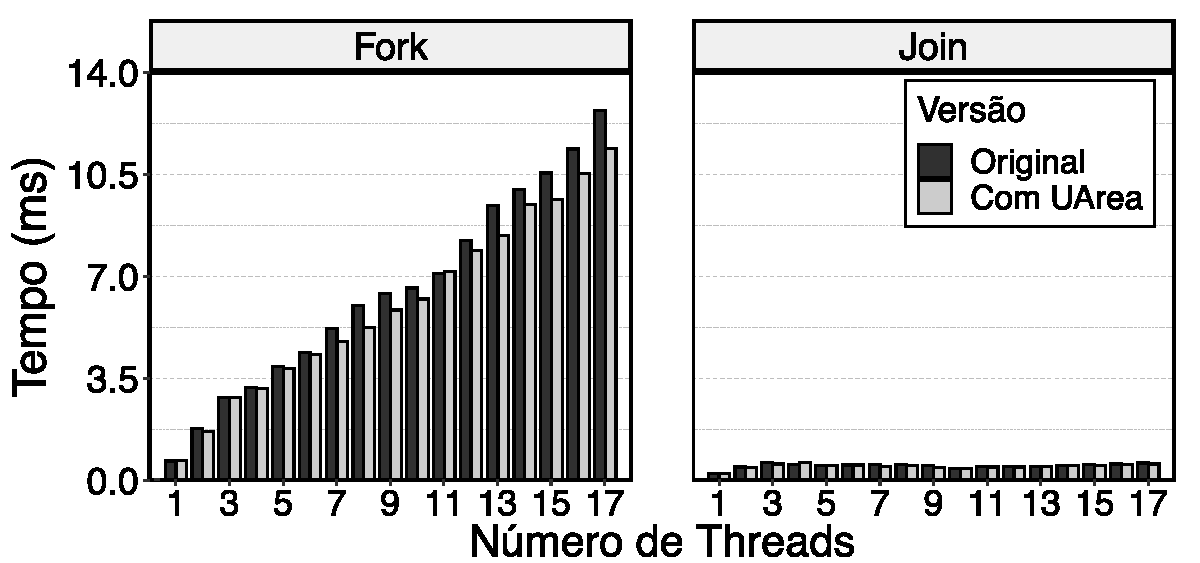
\includegraphics[width=\textwidth]{content/images/fork-join-kernel-time-bars.pdf}}
	\qquad
	\subcaptionminipage[fig.kernel-counters]
                   {.4\textwidth}
                   {Métricas do \kernel.}
                   {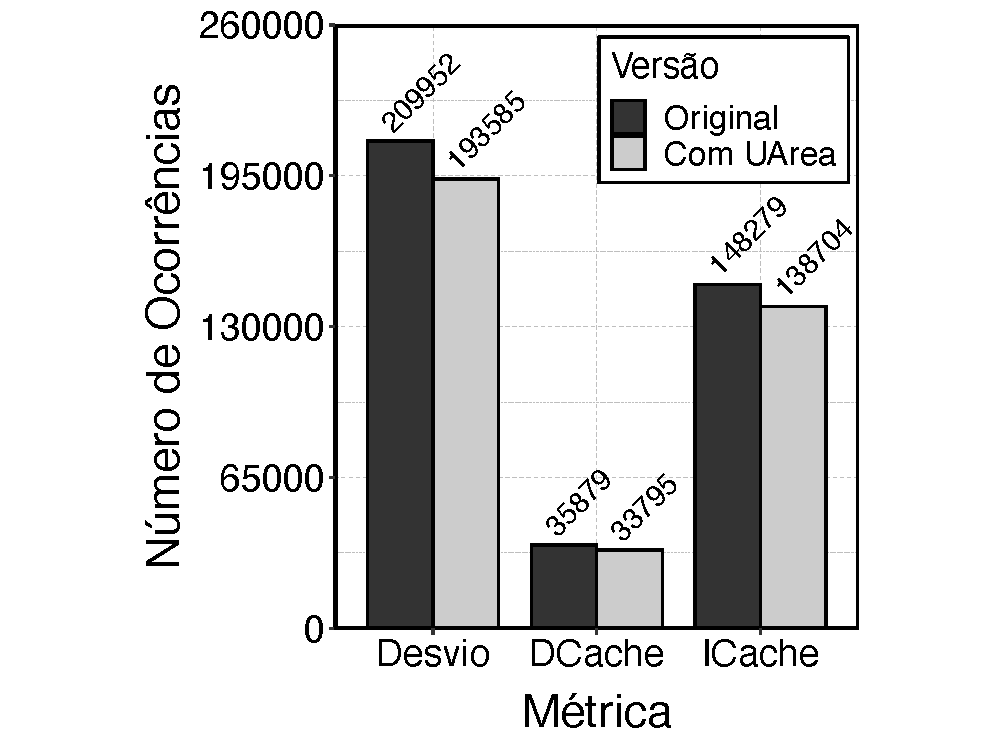
\includegraphics[width=\textwidth]{content/images/fork-join-kernel-counters.pdf}}
	\caption{Impactos da virtualização sobre a manipulação de \threads.\label{fig.threads}}%
\end{figure}

\begin{figure}[tb]
    \centering
    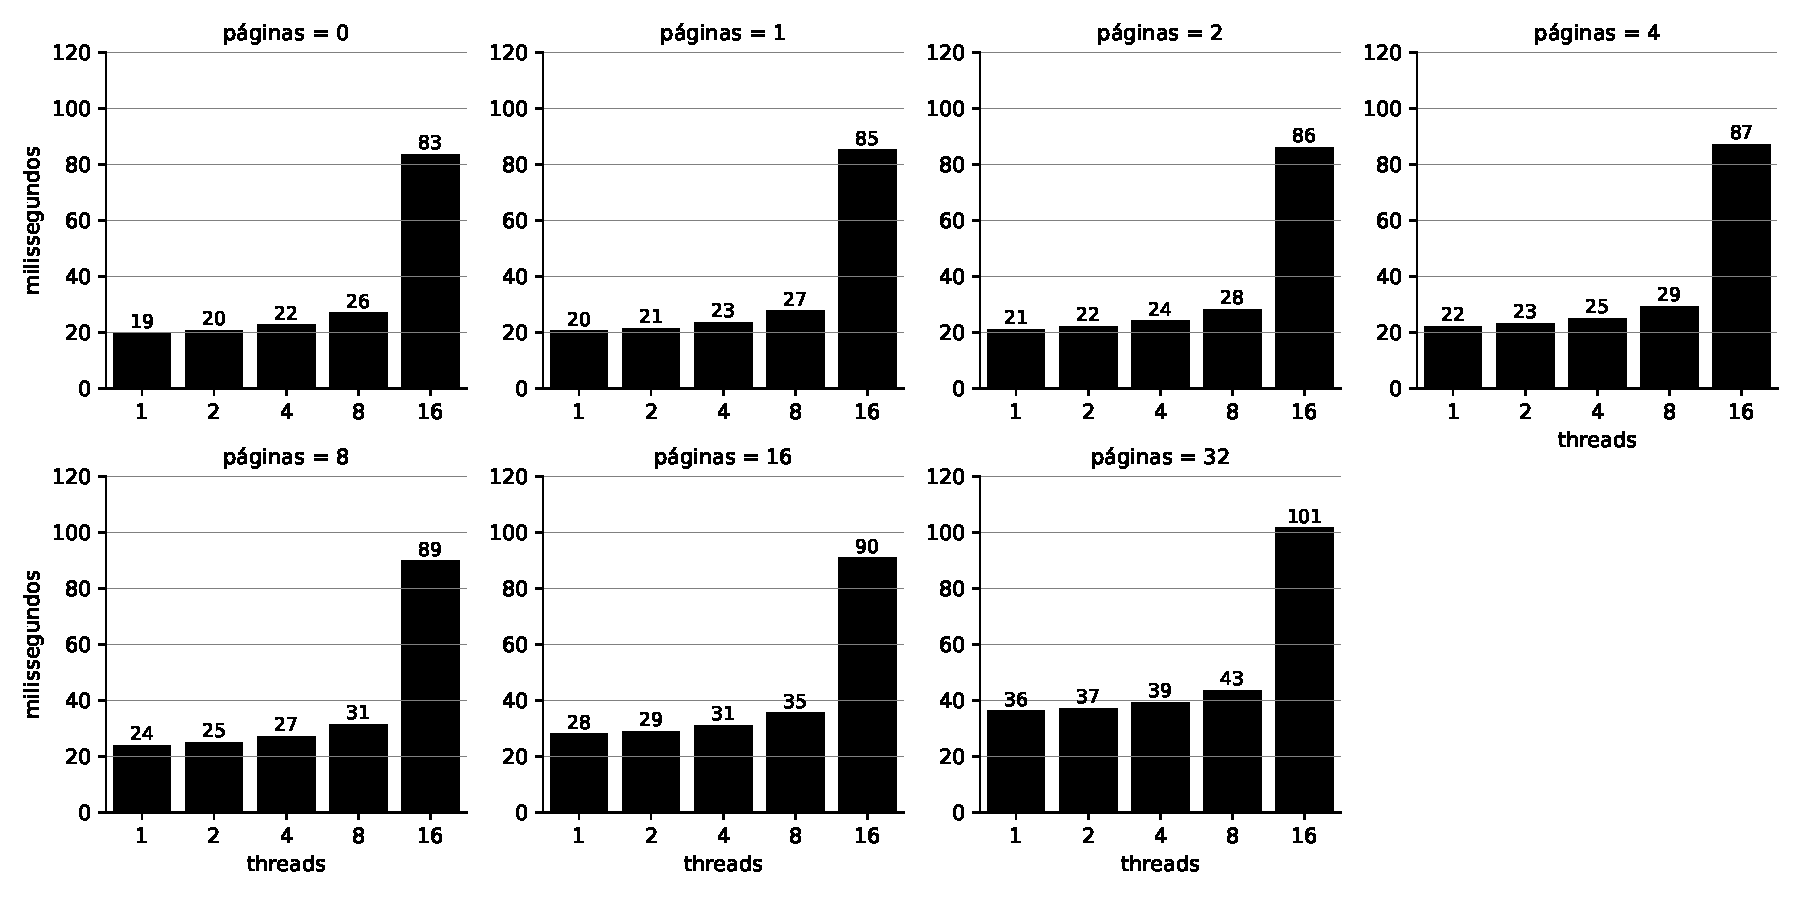
\includegraphics[width=\linewidth]{content/images/multiple_threads_pages.pdf}
    \caption{\Downtime da aplicação durante o experimento de migração fixando a quantidade de páginas alocadas dinamicamente}
    \label{fig.mtpages}
\end{figure}

\begin{figure}[tb]
    \centering
    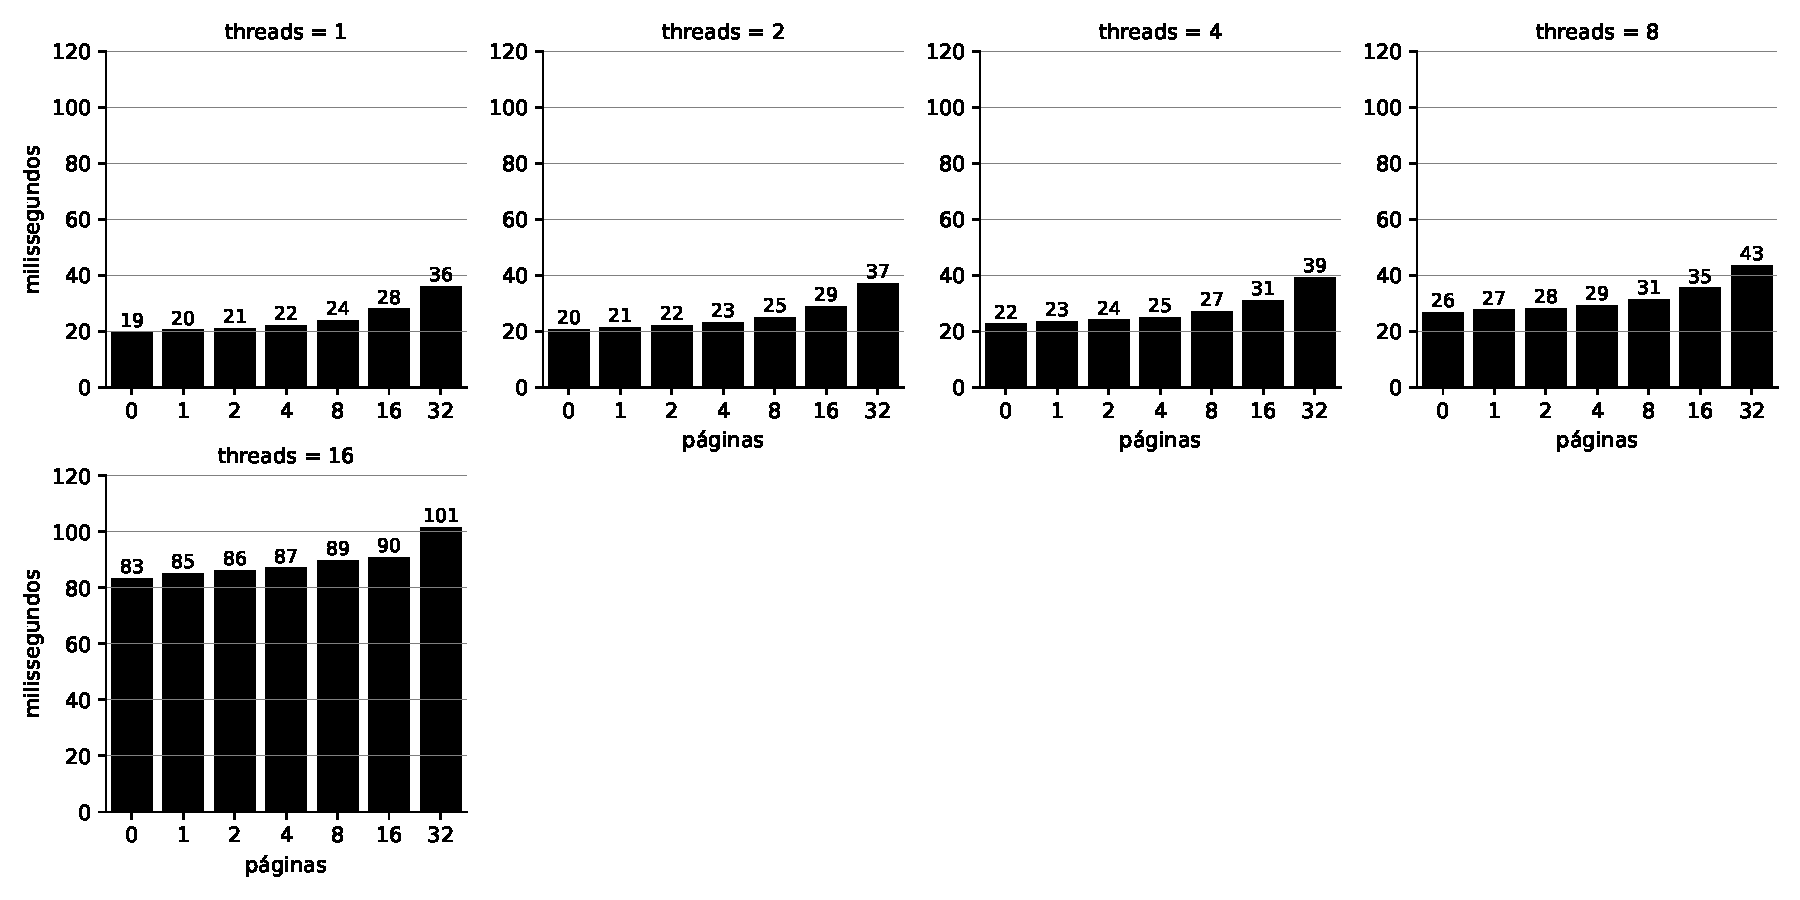
\includegraphics[width=\linewidth]{content/images/multiple_threads_threads.pdf}
    \caption{\Downtime da aplicação durante o experimento de migração fixando a quantidade de \threads}
    \label{fig.mtthreads}
\end{figure}

O primeiro experimento, o qual mensurava o impacto do isolamento da aplicação através da \uarea e separação do binário de usuário e \kernel, mostrou que o subsistema de \threads foi positivamente afetado. A \autoref{fig.fork-join} ilustra que o \nanvix obteve um leve ganho de desempenho nas operações de criação e junção de \threads. A \autoref{fig.kernel-counters} mostra a origem do aumento da performance. Percebemos que houve uma diminuição na quantidade de faltas em \cache (tanto de dados como de instruções) e a quantidade de desvios é menor na versão do \nanvix com a \uarea. Isso ocorre porque a \uarea explora melhor a localidade espacial dos dados, já que os dados estão aglomerados em um espaço menor da memória. Como consequência disso, o número de faltas na \cache e de desvios diminui, resultando em um aumento de desempenho.

O segundo experimento, que mensura o \downtime da aplicação em cenários variando a quantidade de recursos utilizados, mostrou os seguintes resultados. A \autoref{fig.mtpages} e a \autoref{fig.mtthreads} mostram a progressão de tempo sobre diferentes perspectivas (fixando-se as páginas e \threads, respectivamente). Como o esperado, o \downtime aumenta quanto maior for o número de páginas e \threads. Além disso, a quantidade de \threads se destaca por apresentar maior expressividade no tempo contabilizado em comparação com a quantidade de páginas. Isso acontece porque uma \thread acarreta em mais dados migrados do que uma página. De maneira geral, o \downtime é aproximadamente descrito pela função \ref{eq.downtime}:

\begin{equation}\label{eq.downtime}
    \begin{split}
        f(p, t) = \frac{17}{32}*p+t+18
    \end{split}
\end{equation}

Essa função descreve relativamente bem a progressão de tempo até 15 \threads. Como podemos observar nos gráficos, com 16 \threads há uma disparidade com a natureza aparentemente linear que a progressão de tempo aparenta ter. Isso acontece porque o \mppa possui 16 \cores por \cluster, o que significa que simultaneamente apenas 15 \threads de usuário podem executar, já que em um \core executam apenas \threads de sistema, que são responsáveis pelo tratamento de chamadas de sistema e execução das \tasks. Portanto, essa disparidade numérica que os gráficos apresentam são justificados pelo tempo extra que o teste ocupa com gerenciamento de \threads. Isso porque o teste finaliza com a junção de todas as \threads criadas no \cluster destinatário e tal processo exige tempo extra quando a quantidade de \threads é maior que 15, uma vez que algumas \threads precisariam esperar outras terminarem para poderem executar e, finalmente, finalizar sua execução.

O terceiro experimento, que mensurava o \downtime da aplicação quando múltiplas migrações aconteciam simultaneamente, mostrou que a quantidade de migrações paralelas não impacta significativamente o tempo. É importante destacar que nesse experimento foram migradas aplicações que usavam o máximo de recursos de sistema. Mesmo assim, a quantidade de dados não foi suficiente para impactar no \downtime.

Já o quarto experimento, o teste adicional que visava a comprovação da corretude do \daemon, mostrou que: o \daemon é capaz de ser reusado no mesmo \cluster diversas vezes independentemente do papel do \cluster na migração; e que é possível um processo ser migrado diversas vezes para diferentes \clusters, até em movimento circular envolvendo todos os \clusters, como no experimento.